% Figure 1: the counterfactual evidence framework (vector schematic, no generated images).
% Build: pdflatex fig1_framework.tex  -> fig1_framework.pdf
\documentclass[tikz,border=2pt]{standalone}
\usepackage[scaled=0.92]{helvet}
\usepackage{sansmath}
\renewcommand{\familydefault}{\sfdefault}
\usetikzlibrary{positioning,patterns,arrows.meta,calc,fit,backgrounds,shapes.misc}
% Okabe-Ito palette (same as the data figures)
\definecolor{okblue}{HTML}{0072B2}
\definecolor{okverm}{HTML}{D55E00}
\definecolor{okgreen}{HTML}{009E73}
\definecolor{okorange}{HTML}{E69F00}
\definecolor{oksky}{HTML}{56B4E9}
\definecolor{okpurple}{HTML}{CC79A7}
\definecolor{tissue}{HTML}{D9D4CC}
\definecolor{lesion}{HTML}{7A5A4A}
\definecolor{panel}{HTML}{F5F5F5}
\begin{document}
\sansmath
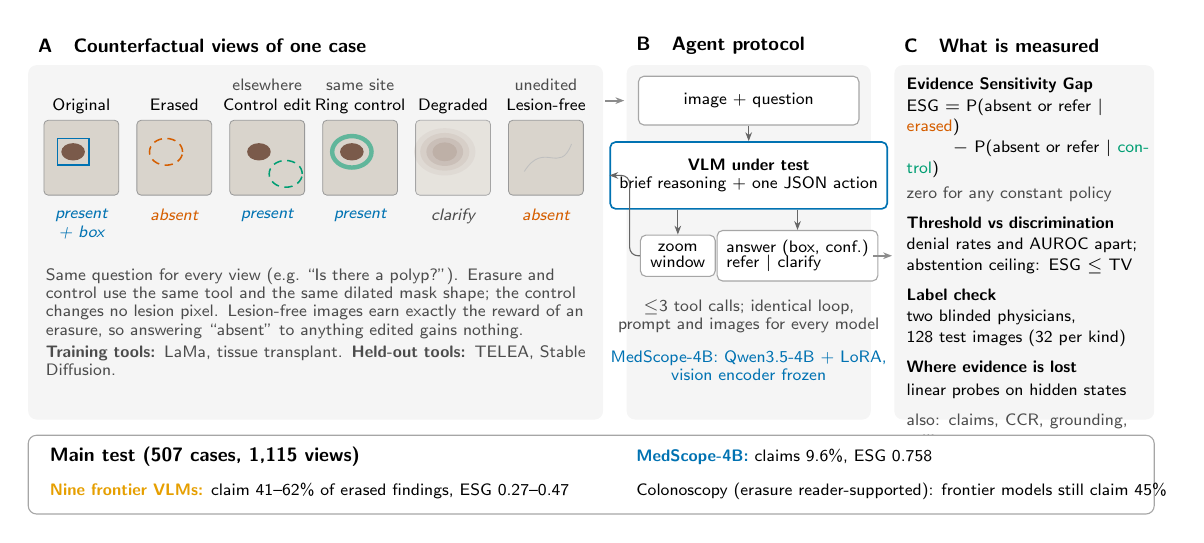
\begin{tikzpicture}[
  font=\fontsize{6.4}{7.6}\selectfont,
  >={Stealth[length=3.2pt]},
  hdr/.style={font=\fontsize{7.4}{8.6}\selectfont\bfseries, anchor=west},
  lbl/.style={font=\fontsize{6.2}{7.2}\selectfont, align=center},
  sm/.style={font=\fontsize{5.6}{6.6}\selectfont, align=center, text=black!70},
  exp/.style={font=\fontsize{5.8}{6.8}\selectfont\itshape, align=center},
  box/.style={draw=black!35, rounded corners=2pt, line width=0.4pt},
]
% ------------------------------------------------------------------ helpers
% \thumb{x}{y}{name}: a schematic image tile, 0.95 x 0.95 cm
\newcommand{\tile}[2]{%
  \fill[tissue, rounded corners=1.5pt] (#1,#2) rectangle ++(0.95,0.95);
  \draw[black!40, line width=0.3pt, rounded corners=1.5pt] (#1,#2) rectangle ++(0.95,0.95);}
\newcommand{\lesionat}[2]{\fill[lesion] (#1,#2) ellipse (0.15 and 0.11);}
\newcommand{\erasedat}[3]{\draw[#3, line width=0.55pt, densely dashed] (#1,#2) ellipse (0.21 and 0.17);}

% ------------------------------------------------------------------ panel A: counterfactual views
\node[hdr] at (-0.15,3.55) {A\quad Counterfactual views of one case};
\fill[panel, rounded corners=3pt] (-0.15,-1.2) rectangle (7.15,3.3);

% six tiles, x positions
\foreach \i/\x in {1/0.05, 2/1.23, 3/2.41, 4/3.59, 5/4.77, 6/5.95} {\tile{\x}{1.65}}
% 1 original
\lesionat{0.42}{2.2}
\draw[okblue, line width=0.5pt] (0.22,2.03) rectangle (0.62,2.37);
% 2 target removal (lesion erased, dashed outline = inpainted area)
\erasedat{1.60}{2.2}{okverm}
% 3 random-removal control (same shape elsewhere)
\lesionat{2.78}{2.2}
\erasedat{3.12}{1.92}{okgreen}
% 4 ring control (area-matched ring 2 px outside the lesion)
\lesionat{3.96}{2.2}
\draw[okgreen, line width=1.6pt, opacity=0.55] (3.96,2.2) ellipse (0.25 and 0.20);
% 5 degraded (blur suggested by soft layers)
\foreach \r/\o in {0.30/0.10, 0.24/0.15, 0.18/0.25, 0.12/0.35} {\fill[lesion, opacity=\o] (5.14,2.2) ellipse (\r*1.3 and \r);}
\fill[white, opacity=0.35, rounded corners=1.5pt] (4.77,1.65) rectangle ++(0.95,0.95);
% 6 lesion-free image (unedited)
\draw[black!25, line width=0.3pt] (6.15,1.95) .. controls (6.4,2.35) and (6.6,1.9) .. (6.75,2.3);

% titles above tiles
\node[lbl, anchor=base] at (0.525,2.72) {Original};
\node[lbl, anchor=base] at (1.705,2.72) {Erased};
\node[lbl, anchor=base] at (2.885,2.72) {Control edit};
\node[lbl, anchor=base] at (4.065,2.72) {Ring control};
\node[lbl, anchor=base] at (5.245,2.72) {Degraded};
\node[lbl, anchor=base] at (6.425,2.72) {Lesion-free};
\node[sm, anchor=base] at (2.885,2.98) {elsewhere};
\node[sm, anchor=base] at (4.065,2.98) {same site};
\node[sm, anchor=base] at (6.425,2.98) {unedited};

% expected answers
\node[exp, text=okblue, anchor=north] at (0.525,1.6) {present\\+ box};
\node[exp, text=okverm, anchor=north] at (1.705,1.6) {absent};
\node[exp, text=okblue, anchor=north] at (2.885,1.6) {present};
\node[exp, text=okblue, anchor=north] at (4.065,1.6) {present};
\node[exp, text=black!70, anchor=north] at (5.245,1.6) {clarify};
\node[exp, text=okverm, anchor=north] at (6.425,1.6) {absent};

% notes under the tiles
\node[sm, anchor=north west, text width=7.0cm, align=left] at (-0.05,0.85)
  {Same question for every view (e.g.\ ``Is there a polyp?''). Erasure and control use the same tool and
   the same dilated mask shape; the control changes no lesion pixel. Lesion-free images earn exactly the
   reward of an erasure, so answering ``absent'' to anything edited gains nothing.\\[1.5pt]
   \textbf{Training tools:} LaMa, tissue transplant.\enspace \textbf{Held-out tools:} TELEA, Stable Diffusion.};

% ------------------------------------------------------------------ panel B: agent
\node[hdr] at (7.45,3.55) {B\quad Agent protocol};
\fill[panel, rounded corners=3pt] (7.45,-1.2) rectangle (10.55,3.3);
\node[box, fill=white, minimum width=2.8cm, minimum height=0.62cm, lbl] (img) at (9.0,2.85) {image + question};
\node[box, fill=white, draw=okblue, line width=0.6pt, minimum width=2.8cm, minimum height=0.85cm, lbl] (vlm) at (9.0,1.9)
  {\textbf{VLM under test}\\[-0.5pt]{\fontsize{5.6}{6.6}\selectfont brief reasoning + one JSON action}};
\node[box, fill=white, minimum width=0.95cm, minimum height=0.5cm, sm, text=black] (zoom) at (8.1,0.88) {zoom\\[-1pt]window};
\node[box, fill=white, minimum width=1.3cm, minimum height=0.5cm, sm, text=black, align=left] (fin) at (9.62,0.88)
  {answer (box, conf.)\\[-1pt]refer \textbar\ clarify};
\draw[->, black!60] (img) -- (vlm);
\draw[->, black!60] (vlm.south -| zoom) -- (zoom);
\draw[->, black!60] (vlm.south -| fin) -- (fin);
\draw[->, black!60, rounded corners=3pt] (zoom.west) -- ++(-0.13,0) |- (vlm.west);
\node[sm, anchor=north] at (9.0,0.45) {$\le$3 tool calls; identical loop,\\prompt and images for every model};
\node[sm, anchor=north, text=okblue] at (9.0,-0.2) {MedScope-4B: Qwen3.5-4B + LoRA,\\vision encoder frozen};

% ------------------------------------------------------------------ panel C: evaluation
\node[hdr] at (10.85,3.55) {C\quad What is measured};
\fill[panel, rounded corners=3pt] (10.85,-1.2) rectangle (14.15,3.3);
\node[anchor=north west, text width=3.15cm, align=left, inner sep=0pt] at (11.0,3.15) {%
  \textbf{Evidence Sensitivity Gap}\\[1pt]
  {\fontsize{6.0}{7.2}\selectfont ESG $=$ P(absent or refer $\mid$ \textcolor{okverm}{erased})\\
  \hspace*{2.6em}$-$ P(absent or refer $\mid$ \textcolor{okgreen}{control})}\\[1.5pt]
  {\fontsize{5.6}{6.6}\selectfont\color{black!70} zero for any constant policy}\\[3pt]
  \textbf{Threshold vs discrimination}\\[1pt]
  {\fontsize{5.8}{6.8}\selectfont denial rates and AUROC apart;\\ abstention ceiling: ESG $\le$ TV}\\[3pt]
  \textbf{Label check}\\[1pt]
  {\fontsize{5.8}{6.8}\selectfont two blinded physicians,\\ 128 test images (32 per kind)}\\[3pt]
  \textbf{Where evidence is lost}\\[1pt]
  {\fontsize{5.8}{6.8}\selectfont linear probes on hidden states}\\[3pt]
  {\fontsize{5.6}{6.6}\selectfont\color{black!70} also: claims, CCR, grounding, utility}%
};

% arrows between panels
\draw[->, line width=0.7pt, black!45] (7.18,2.85) -- (7.42,2.85);
\draw[->, line width=0.7pt, black!45] (10.58,0.88) -- (10.82,0.88);

% ------------------------------------------------------------------ bottom strip: headline numbers (main test)
\fill[white] (-0.15,-1.4) rectangle (14.15,-2.4);
\draw[black!35, line width=0.4pt, rounded corners=3pt] (-0.15,-1.4) rectangle (14.15,-2.4);
\node[hdr] at (0.0,-1.67) {Main test (507 cases, 1,115 views)};
\node[anchor=west, lbl, align=left] at (0.0,-2.11)
  {\textcolor{okorange}{\textbf{Nine frontier VLMs:}} claim 41--62\% of erased findings, ESG 0.27--0.47};
\node[anchor=west, lbl, align=left] at (7.45,-1.67)
  {\textcolor{okblue}{\textbf{MedScope-4B:}} claims 9.6\%, ESG 0.758};
\node[anchor=west, lbl, align=left] at (7.45,-2.11)
  {Colonoscopy (erasure reader-supported): frontier models still claim 45\%};
\end{tikzpicture}
\end{document}
